\documentclass{standalone}
\usepackage{tikz}
\usetikzlibrary{positioning,decorations.pathreplacing}
\begin{document}
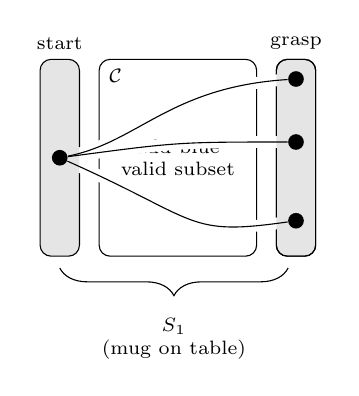
\begin{tikzpicture}[font=\scriptsize]


\node[draw,black,rounded corners,minimum height=2.5cm,minimum width=0.5cm]
   (qstart) at (3,0) {};

\node[draw,black,rounded corners,minimum height=2.5cm,minimum width=0.5cm]
   (Sstart) at (0,0) {};
\node[draw,black,rounded corners,minimum height=2.5cm,minimum width=0.5cm]
   (Sgrasp) at (3,0) {};
   
\node[draw,black,rounded corners,minimum height=2.5cm,minimum width=2cm]
   (S1) at (1.5,0) {};

\node[circle,fill=black,inner sep=2] (xstart) at (0,0) {};
\node[circle,fill=black,inner sep=2] (xg1) at (3,1.0) {};
\node[circle,fill=black,inner sep=2] (xg2) at (3,0.2) {};
\node[circle,fill=black,inner sep=2] (xg3) at (3,-0.8) {};

\node[align=center] at (1.5,0) {add blue\\valid subset};

%\node[above=0.1cm of xstart] {$q_{\mbox{\scriptsize start}}$};
\node[above=0cm of Sstart] {start};
\node[above=0cm of Sgrasp] {grasp};
%\node[above=0cm of S1] {$S_{\mbox{\scriptsize step1}}$};
\node[above left=-0.6cm of S1] {$\mathcal{C}$};

\draw[line width=1.5mm,white]
   (xstart)
   .. controls (1,0.2) and (1.4,0.9) .. (xg1);
\draw[line width=1.5mm,white]
   (xstart)
   .. controls (1.5,0.2) .. (xg2);
\draw[line width=1.5mm,white]
   (xstart)
   .. controls (1.8,-0.8) and (1.6,-1.0) .. (xg3);

\draw
   (xstart)
   .. controls (1,0.2) and (1.4,0.9) .. (xg1);
\draw
   (xstart)
   .. controls (1.5,0.2) .. (xg2);
\draw
   (xstart)
   .. controls (1.8,-0.8) and (1.6,-1.0) .. (xg3);

\node[fill,black,rounded corners,minimum height=2.5cm,minimum width=0.5cm,
   opacity=0.1] at (0,0) {};
\node[fill,black,rounded corners,minimum height=2.5cm,minimum width=0.5cm,
   opacity=0.1] at (3,0) {};

\draw [decorate,decoration={brace,mirror,amplitude=10pt}]
(0.0,-1.4) -- (2.9,-1.4) node [black,midway,yshift=-0.9cm,align=center]
   {$S_1$\\(mug on table)};


\end{tikzpicture}%
\end{document}
